

%\newpage
%\setcounter{page}{1}
\begin{center}
\begin{figure}
\centering%

\epsfig{file=HojaTitulo/EscudoUN.eps,scale=1}%
\end{figure}
\thispagestyle{empty} \vspace*{1.5cm} \textbf{\huge
An\'{a}lisis tridimensional de equilibrio l\'{i}mite por movimientos en masa para la cuenca hidrogr\'{a}fica de la quebrada La Linda en la vereda Monte Loro en Ciudad Bolivar (Antioquia) mediante el programa Scoops 3D}\\[4.0cm]
\Large\textbf{Juan Felipe Luj\'{a}n Rivas}\\[4.0cm]
\small Universidad Nacional de Colombia\\
Facultad de Minas, Departamento de ingenier\'{i}a Civil \\
Medell\'{i}n, Colombia\\
2019\\
\end{center}

\newpage{\pagestyle{empty}\cleardoublepage}

\newpage
\begin{center}
\thispagestyle{empty} \vspace*{0cm} \textbf{\huge
An\'{a}lisis tridimensional de equilibrio l\'{i}mite por movimientos en masa para la cuenca hidrogr\'{a}fica de la quebrada La Linda en la vereda Monte Loro en Ciudad Bolivar (Antioquia) mediante el programa Scoops 3D}\\[2.0cm]
\Large\textbf{Juan Felipe Luj\'{a}n Rivas}\\[2.0cm]
\small Tesis o trabajo de grado presentada(o) como requisito parcial para optar al
t\'{\i}tulo de:\\
\textbf{ Magister en Ingenier\'{\i}a Geotecnia}\\[1.5cm]
Director(a):\\
Ph.D. Ludger O. Suarez. Burgoa\\[1.0cm]
L\'{\i}nea de Investigaci\'{o}n:\\
Estabilidad de Laderas\\
Grupo de Investigaci\'{o}n:\\
Grupo de Investigaci\'{o}n BIMs (Blocks in Matrix)\\[0.5cm]
Universidad Nacional de Colombia\\
Facultad de Minas, Departamento de Ingenier\'{i}a Civil\\
Medell\'in, Colombia\\
2019\\
\end{center}



\newpage
\thispagestyle{empty} \textbf{}\normalsize
\\\\\\%
\addcontentsline{toc}{chapter}{\numberline{}Agradecimientos}\\\\
\begin{figure}[H]
\centering
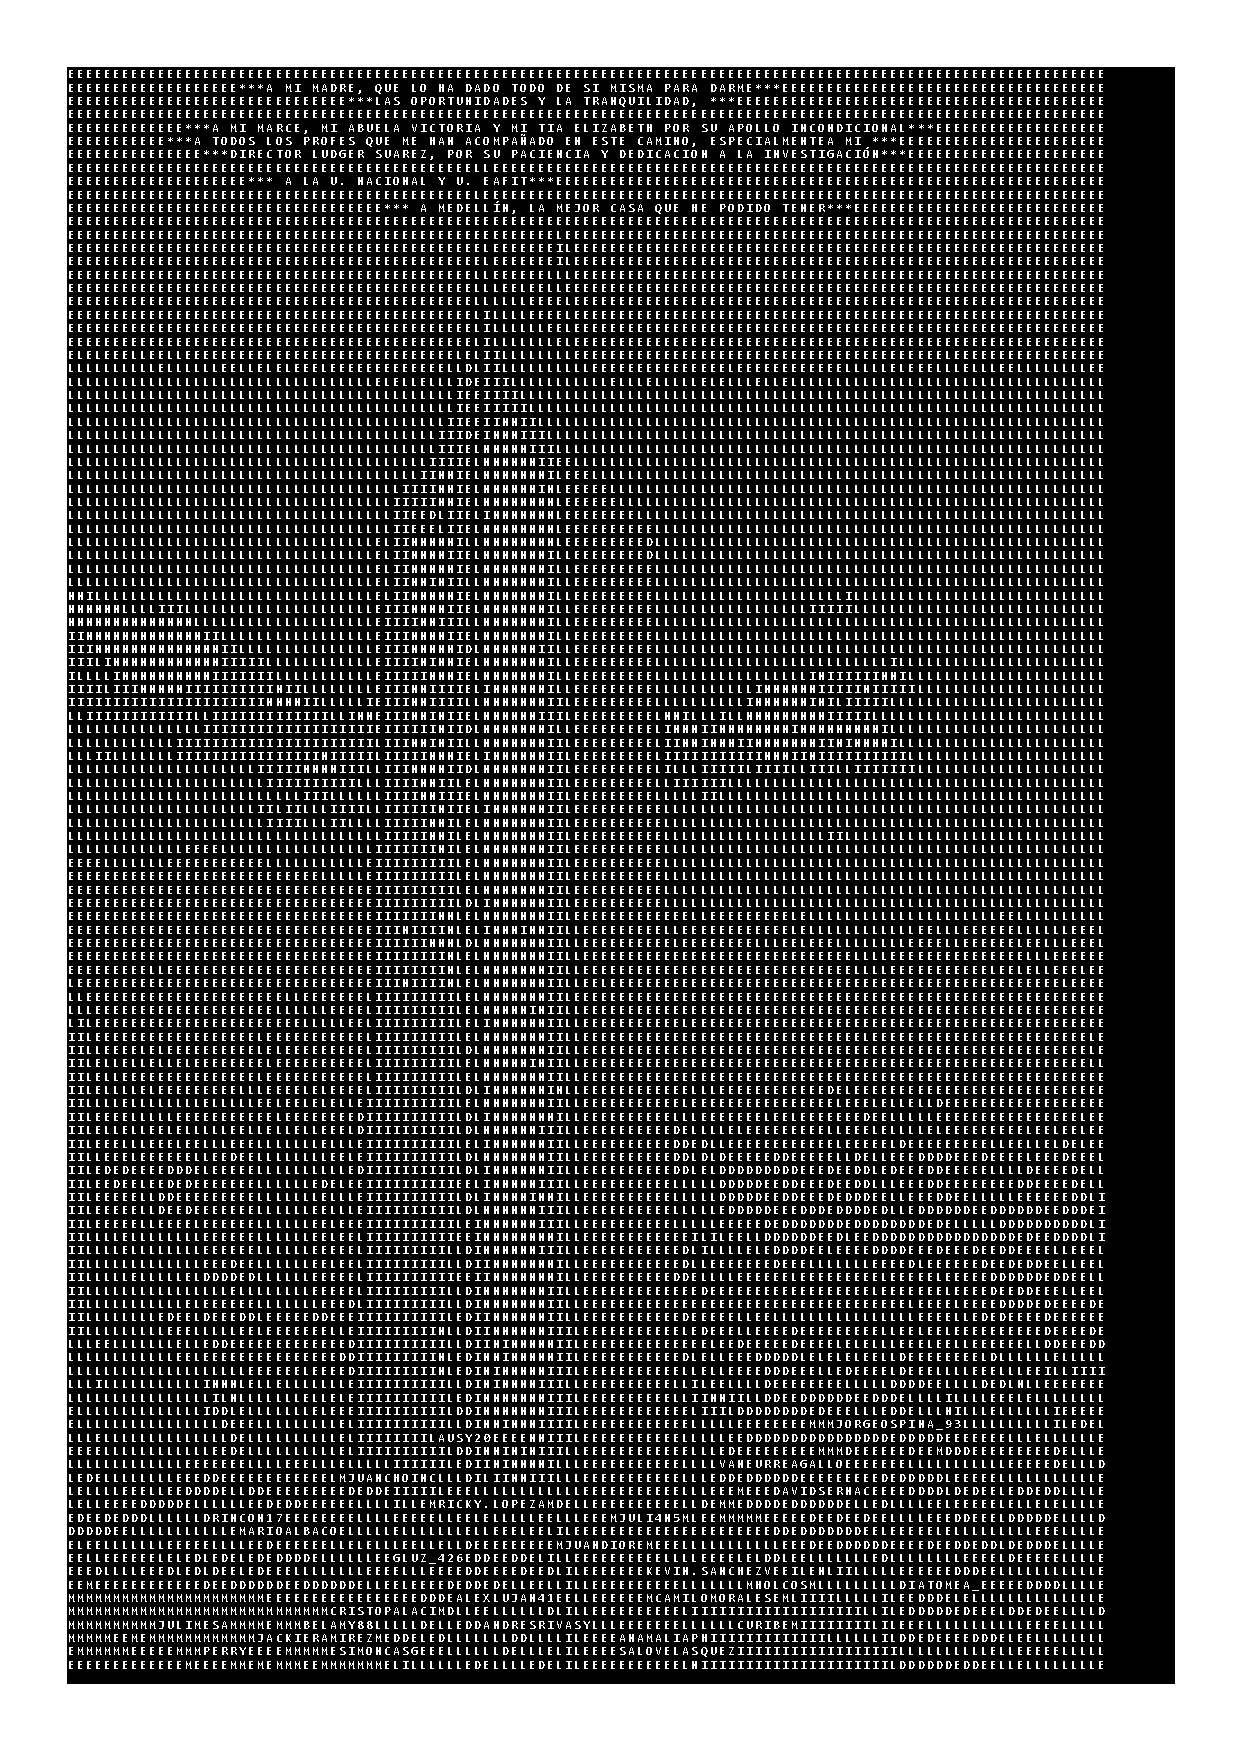
\includegraphics[trim={0 0.1cm 2.2cm 0},clip,scale=0.8]{img/dedicatoria/dedicatoria.pdf}
\end{figure}

\newpage{\pagestyle{empty}\cleardoublepage}

\newpage
\textbf{\LARGE Resumen}\\
En esta investigaci\'on se demuestra la aplicaci\'on de m\'etodos de an\'alisis de equilibrio l\'imite (bishop simplificado), aplicado de manera tridimensional sobre un sector conocido popularmente como Vereda Monteloro, en el municipio de Ciudad Bol\'ivar, Antioquia. Para dicho procedimiento se utilizan como insumos: informaci\'on geogr\'afica y de elevaci\'on contenida en un modelo de elevaci\'on digital (DEM por sus siglas en ingl\'es), par\'ametros de resistencia, espec\'ificamente \'angulo de fricci\'on y cohesion obtenido de ensayos de laboratorio ejecutados sobre muestras recolectadas en la zona de estudio. Como resultado se obtiene un mapa de calor de la zona trabajada en el cual se logra apreciar la distribuci\'on de factores de seguridad (que descienden hasta 1.46) y su correlaci\'on con factores como la pendiente y los mismos par\'ametros de resistencia. Adicionalmente se obtiene informaci\'on cuantitativa, como el total de superficies de falla evaluados \(1\,665\,954\)), as\'i como  vol\'umen y masa estimados del cuerpo de suelo con menor factor de seguridad encontrado, siendo estos valores $211.180\text{m}^{3}$ y $534.24\,\text{kg}$ respectivamente.
Se detalla y ejemplifica el uso de Scoops3D como herramienta computacional para la generaci\'on del mapa de distribuciones de factores de seguridad. 



\newpage
\textbf{\LARGE Abstract}\\
This research demonstrates the application of limit equilibrium analysis methods (simplified bishop), applied in a three-dimensional slope located in Vereda Monteloro, in the municipality of Ciudad Bolivar, Antioquia. For this, the following data will be used as input: geographic and elevation information contained in a digital acceleration model (DEM), and resistance parameters of the soil, specifically the angle of friction and cohesion obtained from laboratory tests carried out on soil samples collected in the study zone. As a result, a heat map of the area is obtained in which it is possible to obtain the distribution of safety factors (going down as low as $1.46$) and its correlation with variables such as the slope and the resistance parameters. Additionally, quantitative information is obtained, such as the total fault surfaces evaluated, 1665954 in this case), as well as the estimated volume and mass of the soil body with the lowest safety factor, these values being 211.180 cubic meters and 534.24 kg respectively. The use of Scoops3D as a computational tool for generating safety factor distribution maps is detailed and exemplified.
\addcontentsline{toc}{chapter}{\numberline{}Resumen}
